
\label{sec:systemArchitecture}

Dieses Kapitel soll ein Gefühl für die Komponenten von \emph{Flewnit} und 
ihre Zusammenhänge vermitteln. Die Komponenten "`in Aktion"' werden im Detail im Verlauf des Kapitels 
\ref{sec:simulation} beschrieben.
Dieses Kapitel soll die groben Konzepte und Ideen teilweise anhand von Beispielen vorstellen.
Nicht jedes Feature, welches erwähnt wird, ist auch tatsächlich vollständig implementiert und getestet.
Über den Status der Implementierung zum Zeitpunkt der Abgabe dieser Ausarbeitung
gebe ich am Ende dieses Kapitels (Abschnitt \ref{sec:statusImplementation}) einen Überblick.

Das System wurde in C++ als (wahlweise statisch oder dynamisch zu linkende) Bibliothek implementiert.
Der Code der GPU-Programme ist in GLSL bzw. OpenCL C verfasst.

\subsection{Dependencies}
	\label{sec:dependencies}
	
	Zunächst sollen die verwendeten Third-Party-Bibliotheken kurz vorgestellt werden:

	\begin{description}
		\item[OpenGL3/4]
		Die schon mehrfach erwähnten modernen Versionen der \linebreak \emph{Open Graphics Library},
		der offenen API der Khronos Group zur \linebreak hardwarebeschleunigten Graphik-Programmierung 
		auf Basis der Dreiecks-Rasterisierung.
		\todo[color=green]{evtl treffenderen Ausdruck finden: Scanline-basiert oder was auch immer}
		Um die Programmierung ohne Legacy-Routinen nicht erst zur Laufzeit über einen OpenCL-Error
		durch Verwendung eines Core-Profiles zu erzwingen, gibt es einen OpenGL- Header
		namens "`gl3.h"'\footnote{beziehbar unter http://www.opengl.org/registry/},
		der in Kombination mit der entsprechenden Präprozessor-Definition
		\lstinline[language=C]|#define GL3_PROTOTYPES 1| schon zur Compile-Zeit nur die non-deprecated
		Routinen zur Verfügung stellt.
		
     	\item[OpenCL 1.0]
	    Die \emph{Open Computing Language}, erste Version der noch jungen API für massiv parallele Programmierung
	    \footnote{die GPGPU-Computing einschließt}, wie OpenGL von der Khronos Group verwaltet; 
	    sie stellt den ersten offenen Standard für GPGPU dar, d.h., die Verwendung der API ist nicht mehr an eine
	    bestimmte Hardware (wie bei Nvidia CUDA) oder ein bestimmtes Betriebssystem (wie Microsofts DirectCompute)
	    gebunden.
	    
	    Zur Zeit der Implementierung waren noch keine Non-Developer-Treiber für OpenCL 1.1 verfügbar, 
	    außerdem gab es kein Feature dieser Version, welches ich dringend benötigt hätte.
	    Deshalb habe ich die Version 1.0 verwendet.
	    
	    Es gibt einen C++ -Wrapper der C-API, welcher stark auf C++-Templates basiert und in einer einzigen Headerdatei 
	    implementiert ist. Dieser ist direkt von der Khronos-Homepage\footnote{http://www.khronos.org/registry/cl/} 	
	    beziehbar. Diesen Wrapper habe ich verwendet, da er die Nutzung der API wesentlich eleganter macht.
	    
    	
   		\item[GLFW 2.7]
		Wie auf Seite \pageref{focus:dependencies} angedeutet, waren mir folgende Dinge wichtig, damit die Einsetzbarkeit
		des Frameworks in professionelleren Kontexten nicht schon im Vorfeld verbaut ist:
		\begin{itemize}
			\item Option auf Fullscreen
			\item Option auf Multisampling
			\item Die Möglichkeit der Erstellung eines OpenGL-Kontextes einer frei wählbaren Version 
			mit Option zwischen Core- und Compatibility-Profile
			\item Option auf "`\emph{Mouse Grab}"', so dass man wie in einem Computerspiel mit ausgeblendetem Mauszeiger
			nur durch Bewegung der Maus ohne Bildschirm-/Fenster-Grenzen die virtuelle Kamera rotieren kann;
			\item "`Input events"', d.h. Aktualisierungen von Benutzereingaben sollen häufig und mit minimaler 
			Latenz geschehen, außerdem so unabhängig wie möglich von der Framerate sein;
			Nach möglichkeit sollten Input-Updates zumindest "aktiv abfragbar" sein 
			(im Gegensatz zum passiven Warten darauf, dass von der Input-Library eine Callback-Funktion 
			aufgerufen wird)
			\item Es soll volle Kontrolle über die "Render-Loop" geben, so dass man nicht 
			den Kontrollfluss an eine Funktion übergibt, die womöglich nie zurückkehrt und weiteren Kontrollfluss
			durch das Benutzerprogramm	nur über Callback-Funktionen ermöglicht
			(wie \lstinline[language=C]|glutEnterMainLoop()| beim in die Jahre gekommenen \emph{GLUT}).
			Ein derartiges Konstrukt ist einer
			Engine nicht würdig und verhindert womöglich sauberes Herunterfahren und Neu-Initialisierung,
			wie es z.B. beim Wechseln einer Szene oder eines fundamentalen globalen Settings nötig sein könnte.	
		\end{itemize}
		\emph{GLFW}\footnote{http://www.glfw.org/} in der Version 2.7, die zum Zeitpunkt der Implementation aktuellste 
		stabile	Version, erfüllt diese Forderungen, und findet damit in \emph{Flewnit} Einsatz sowohl im Fenster- als auch 	
		im Input-Manager. Die Timing-Funktionalität wird ebenfalls von GLFW übernommen.
		
    	
    	\item[OpenGL Mathematics (GLM)]
    	Seit sämtlicher Mathematik-bezogener OpenGL-State inklusive zugehöriger built-in-Variablen und -Funktionen
    	wie \lstinline[language=GLSL]|gl_ModelViewProjectionMatrix| oder
    	\lstinline[language=GLSL]|ftransform()|
    	in GLSL abgeschafft wurden, führt um eine Bibliothek für Vektor- und Matrix-Algebra kein Weg mehr herum.
    	Ich habe mich für \emph{GLM}\footnote{http://glm.g-truc.net/} entschieden, da sie klein und dennoch mächtig ist,
    	und einige Convenience-Functions hat; QT hat ebenfalls eine Mathe-Bibliothek, verwendet jedoch
    	\lstinline[language=C]|double|, also 64bit-Fließkomma-Werte als Basis-Datentyp, was das direkte Übergeben
    	als Array von \lstinline[language=C]|float|-Uniforms an die OpenGL-Shader verhindert. Zwar unterstützen OpenGL
    	und moderne Graphikkarten \lstinline[language=C]|double| nativ, jedoch mit drastisch geringerer Geschwindigkeit,
    	da weniger Recheneinheiten für diesen Datentypen zur Vervügung stehen.\\
    	Es sei bemerkt, dass ich persönlich die direkte Verwendung einer C++ - Mathe-Bibiothek mit überladenen Operatoren
    	und eigener Akkumulation von Matrizen wesentlich angenehmer und eleganter finde als das zähe Hantieren
    	mit der C-API zum modifizieren des OpenGL-State mit seinen Matrix-Modes.
    	
    	\item[Grantlee]
	 		\lstset{language=GLSL} 
       		Die bereits erwähnte Template-Engine; die Syntax entspricht der der Template-Sprache des 
       		\emph{Django} web Frameworks\footnote{https://www.djangoproject.com/}.\\

       		Es lassen sich durch die Applikation Werte an die Template-Engine übergeben, anhand derer
       		dann die Code-Generierung Kontrolliert wird, bzw welche durch durch Einschluss in doppelte
       		geschwungene Klammern direkt eingefügt werden können. \\
       		Beipiel:
			\begin{lstlisting}      		
vec4 fragmentColor =  	
	  
		texture(decalTexture,input.texCoords.xy);
	 color;
	  
			\end{lstlisting} 
			\begin{lstlisting}
#define NUM_BITS_PER_KEY_TO_SORT ( {{numBitsPerKey}} )
			\end{lstlisting} 
     		
       		Die Engine stellt einen Vererbungs-Mechanismus bereit:\\
       		Auf diese Weise kann z.B. die Datei "`particleSimulationTemplate.cl"' verschiedene "`Code-Blocks"'
       		definieren wie z.B.
       		
       		\begin{lstlisting}

	
	the core of the physics simulation: 
	accumulate all relevant values 
	(density, pressure force, viscosity force etc ...)
	               

       		\end{lstlisting}
       		
       		, die von anderen Datein geerbt und entsprechend angepasst implementiert werden.\\
       		"`updateDensity.cl"' erbt von dieser Datei durch die Directive
       		\lstinline[language=GLSL]|| 
       		und implementiert die Dichte-Berechnungen, 
       		ohne dass der umschließende (nicht unerheblich lange und komplexe) Kontrollfluss-Code wiederholt werden muss:
       		\begin{lstlisting}

	if( BELONGS_TO_FLUID(
			GET_CURRENT_NEIGHBOUR_PARTICLE_OBJECT_ID  ) )
	{
		ownDensity +=                   
			cObjectGenericFeatures [ GET_CURRENT_NEIGHBOUR_PARTICLE_OBJECT_ID  ].massPerParticle
			* poly6( ownPosition -  GET_CURRENT_NEIGHBOUR_POS , cSimParams );
	}

       		\end{lstlisting}

       		
       		
    	\item[Assimp]
    	Die \emph{Open Asset Import Library}\footnote{http://assimp.sourceforge.net/} ermöglicht das Auslesen
    	von Szenen direkt aus .blend-Dateien, dem nativen Datenformat des exzellenten Free Software -- 3D-
    	Modellierungsprogramms \emph{Blender}\footnote{http://www.blender.org/}.
    	Somit entfällt der Umständliche Export in ein Zwischenformat.

    	
   		\item[TinyXML]
   		Um zu gewährleisten, dass das System schon in der frühen Entwicklungsphase weitgehend ohne 
   		Recompile-benötigenden "`Hard-Codes"' konfigurierbar ist, wurde TinyXML verwended, um eine XML-
   		config-Datei zu parsen.    	
    
	
	\end{description}	

	Außerdem haben manche Komponenten der \emph{Boost}-Libraries\footnote{http://www.boost.org/} verwendet.
	
	


\subsection{Klassendiagramm}

\begin{figure}[!h]
	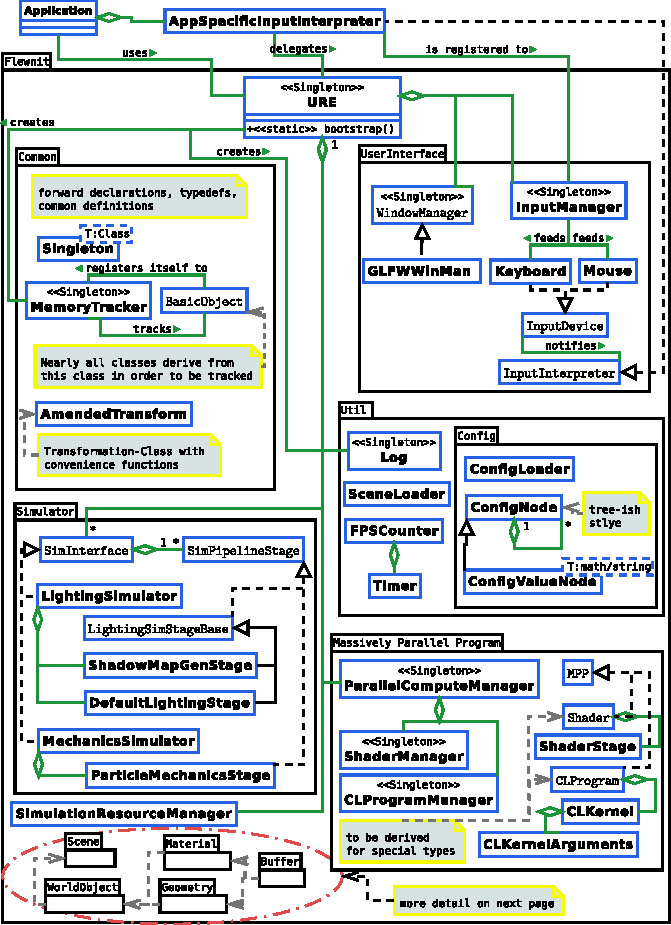
\includegraphics[width=1.09\textwidth]{Overview_Flewnit_Architecture_After_Implementation1.pdf}
	%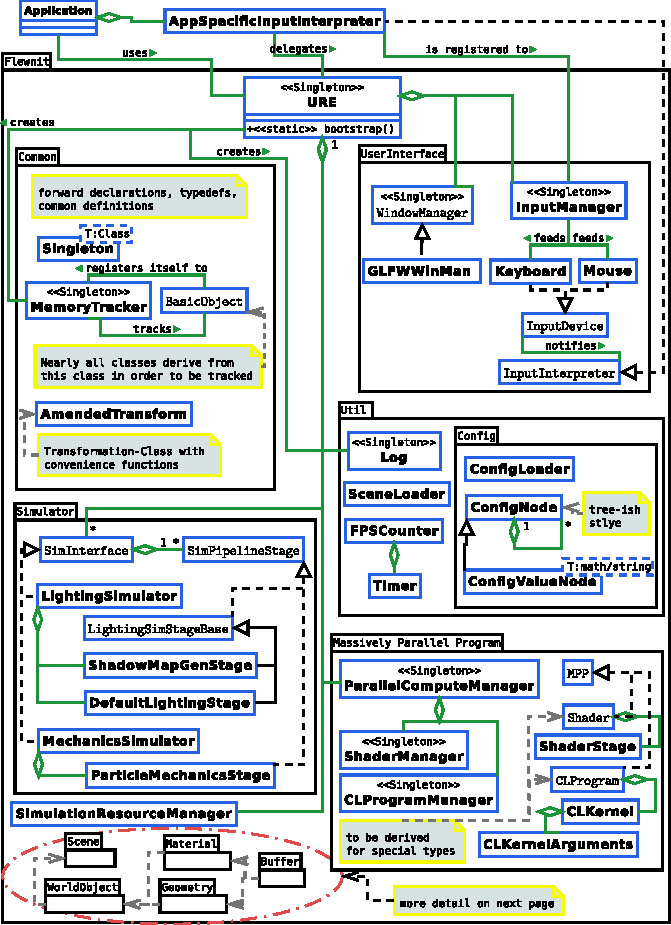
\includegraphics[width=\textwidth]{Overview_Flewnit_Architecture_After_Implementation1.pdf}
	\caption{Klassendiagramm des Gesamtsystems, Teil 1}
	\label{fig:ClassDiagOverview1}
\end{figure}


\begin{figure}[!h]
	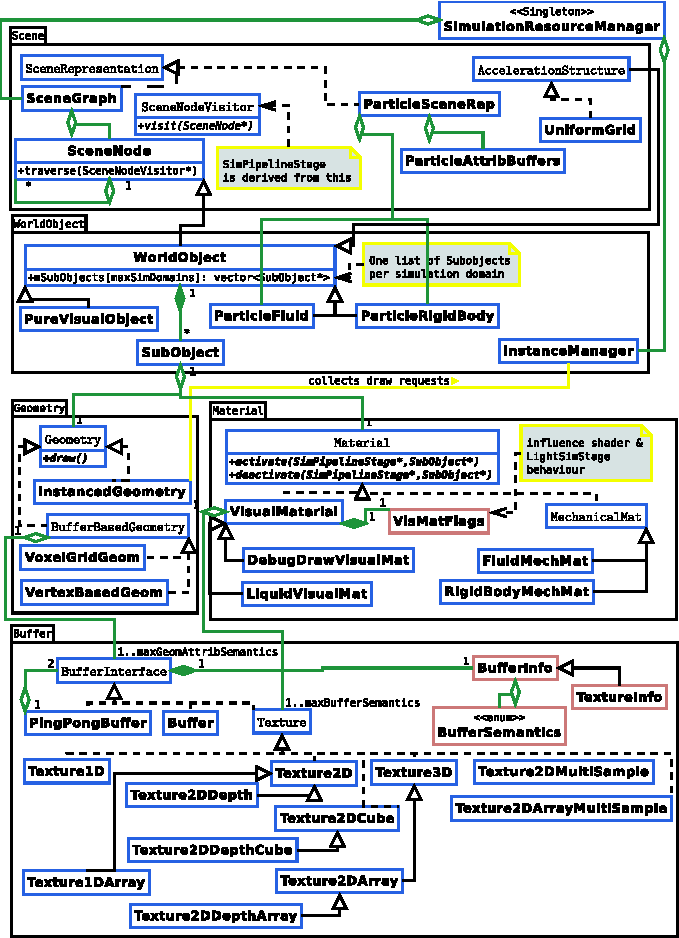
\includegraphics[width=1.09\textwidth]{Overview_Flewnit_Architecture_After_Implementation2.pdf}
	%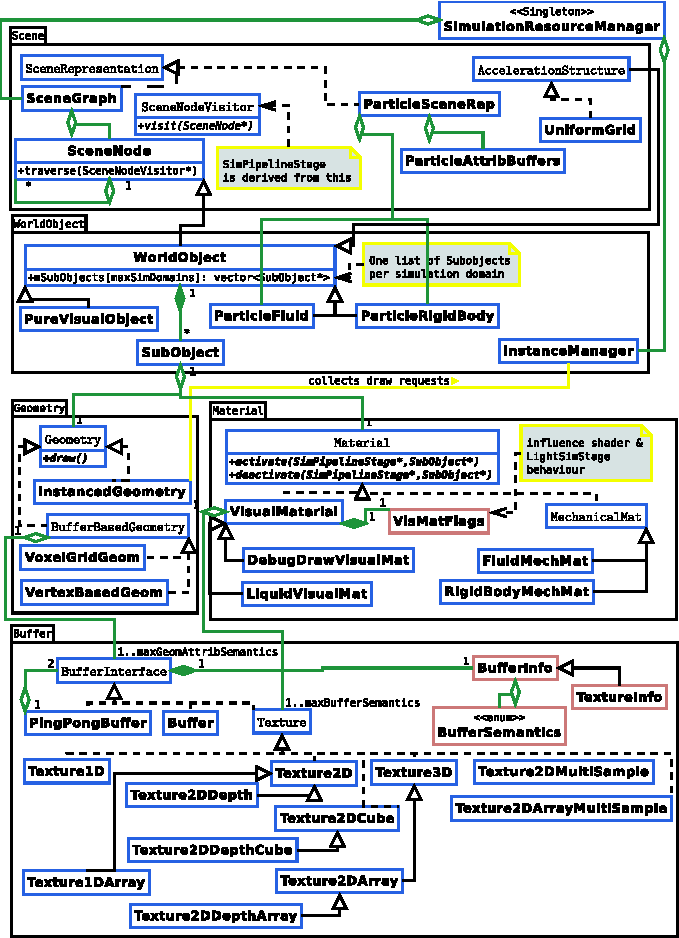
\includegraphics[width=\textwidth]{Overview_Flewnit_Architecture_After_Implementation2.pdf}	
	\caption{Klassendiagramm des Gesamtsystems, Teil 2}
	\label{fig:ClassDiagOverview2}
\end{figure}



Abbildung \ref{fig:ClassDiagOverview1} und \ref{fig:ClassDiagOverview2} zeigen ein vereinfachtes Klassendiagramm
von \emph{Flewnit}. Die roten Klassen stellen wichtige Meta-Informationen dar, um Kontrollfluss und Objekt-Erstellung
zu delegieren. In den folgenden Unterabschnitten werden die einzelnen Komponenten detaillierter vorgestellt.




 
\subsection{BasicObject und Memory Tracking}
	\lstset{language=C++} %we want c++ code listings
	
	Die Bibliothek soll zur Laufzeit kontrolliert herunterfahr- und re-initialisier-bar sein, 
	um eine vielseitige und flexible Anwendung zu gewährleisten. Da bei C++ das Speicher-Management dem
	Programmierer überlassen ist, und man daher vor allem bei massiver Nutzung von Pointern schnell den Überblick
	verliert, 
	\begin{itemize}
		\item welches Objekt welche anderen erschaffen hat
		\item welche Objekte eine Klasse "`besitzt"' und somit für ihre Speicher-Freigabe zuständig ist bzw
		\item auf welche Objekte eine Klasse nur ein Handle für Verwaltung oder	Backtracking hat, ohne für Erschaffung
		 oder Löschung zuständig zu sein
	\end{itemize}
	wurde in Anbetracht der oberen Forderung ein sehr simples Meta-Object-System system realisiert, welches Klassen-Namen
	und Speicherverbrauch eines Objektes feststellt sowie jedem Objekt eine \emph{unique ID} zuweist.
	Zweck dieses Meta Object System-Systems war es, Speicherlecks durch Nicht-Löschen von Objekten während der Entwicklung 
	zu finden;
	
	Dafür erbt beinahe jede Klasse in \emph{Flewnit} von \lstinline|BasicObject|.
	Diese Klasse registriert sich automatisch bei der \lstinline|MemoryTracker|-Singleton-Instanz, bekommt dort eine
	ID zugewiesen. Diese ID hat noch keine Anwendung, könnte sich aber in einem Netzwerk-Kontext als nützlich erweisen.

	Wie bei Qt das \lstinline[language=C++]|Q_OBJECT|-Makro muss in jede von 
	\lstinline[language=C++]|BasicObject| erbende Klasse das Makro 
	\lstinline[language=C++]|FLEWNIT_BASIC_OBJECT_DECLARATIONS| eingetragen werden; Dieses Makro definiert die 
	Implementatoin einer virtuellen Funktion, welche die Meta-Information setzen:
    \begin{lstlisting}
#define FLEWNIT_BASIC_OBJECT_DECLARATIONS \
	public:\
		virtual void initBasicObject() \
		{ \
			mMemoryFootPrint = (int) sizeof(*this); \
			mClassName = String(typeid(*this).name()); \
		} \
	private:	
	\end{lstlisting}
	Diese umständliche Implementierung hat die Urasache, dass Typ-Informationen der Blatt-Klasse einer
	Klassenhierarchie erst dann zur verfügung stehen, wenn alle Konstruktoren der Basis-Klassen zurückgekehrt sind,
	weshalb der obere Code also nicht im Konstruktor der Basisklasse stehen darf, da der \lstinline|this|-Pointer
	noch nicht die Informationen der Blatt-Klasse enthält.
	Ferner, um dem Programmierer nicht zuzumuten, \lstinline|initBasicObject()| in jedem Konstruktor aufzurufen
	(das führt bei tiefen Klassenhierarchien zu unnötigen ausführungen dieser Funktion, da nur die Info der Blatt-Klasse
	benötigt wird, außerdem entstünde so eine weitere Vergesslichkeits-Fehlerquelle, die durch das Meta Object System ja 
	gerade \emph{vermieden} werden soll), stellt der Memory Tracker eine Routine \lstinline|updateMemoryTrackingInfo()|
	bereit, die aufgerufen werden sollte, wenn man auf valide Meta-Information zugreifen will.
	Aufpassen muss man bei tiefen Klassenhierarchien, da hier der Compiler keinen Fehler erzeugt, wenn eine Blatt-Klasse
	das Makro nicht eingetragen hat, da eine Implementierung der Funktion ja bereits durch eine Oberklasse existiert.
	
	Über bedingte Kompilierung lässt sich diese Meta-Funktionalität deaktivieren.
	Ein "`richtiges"' Meta Object System wie das von Qt wollte ich nicht verwenden, da es für meine Zwecke zu komplex und
	mächtig ist, und ich nicht mit Kanonen auf Spatzen schießen wollte. Ohnehin gibt es Tools wie Valgrind, mit denen
	man Speicherlecks finden kann. 

	Letztendlich ist meine Lösung nicht wirklich elegant (auch wenn ich ohne Meta-Object-Compiler (MOC) keine bessere 	
	Lösung gefunden habe) und daher eher als eine Spielerei anzusehen
	mit dem Zwecke, die C++-Interna zu verinnerlichen und zu jeder Zeit daran erinnert zu werden, 
	Destruktoren zu implementieren und sich über 
	"`Besitz- und Verwaltungs-Verhältnisse"' der Klassen Gedanken zu machen.
	
	Der \lstinline|MemoryTracker| verfolgt auch sämtliche Allokationen der \lstinline|BufferInterface|-Klasse,
	also der Basisklasse sämtlicher Buffer-Typen;
	
\subsection{AmendedTransform}
	\label{sec:AmendedTransform}
 	Im Zuge der Überlegungen zum Szenegraphen, der Kamera und des visuellen Renderings vieler Objekte per
 	Hardware-Instancing entschied ich mich, die klassische 4x4-Transformationsmatrix zu wrappen und mit
 	convenience functions anzureichern, siehe Listing \ref{listing:AmendedTransformDef}.\\
 	Der Zweck dieser Klasse ist es, Transformationsmatrizen anhand "`anschaulicher"' Parameter 
 	(Position, Richtung, Up-Vektor, Skalierung) zu definieren,
 	und diese Parameter auch nach Akkumulationen, Modifikationen und/oder Animationen zur Verfügung zu haben.\\
 	Der Fokus liegt hier klar auf der Bequemlichkeit für den Entwickler, nicht auf der Performanz.
 	Sobald sehr große, dynamisch animierte und tiefe Scenegraphen zum Einsatz kommen, könnte diese Klasse
 	zum Flaschenhals werden. Dann ist vielleicht ein Refactoring vonnöten; Vorerst scheint mir die Implementation jedoch
 	angemessen.\\
 	
 	So lässt sich z.B. bequem ein \lstinline|Camera|-Objekt, welches selber von \lstinline|WorldObject| erbt,
 	welches wiederum von \lstinline|SceneNode| abgeleitet ist, an eine andere SceneNode anhängen, und aus der automatisch
 	berechneten globalen Transformation erhält man durch \lstinline|AmendedTransform::getLookAtMatrix()|
 	direkt die lookAt-Matrix, so  dass die Camera-Klasse selber sich nur noch um seine Projektionsmatrix kümmern muss.
 	Auch typische Animationen werden von der Klasse übernommen. Ob dies guter Stil ist, oder doch lieber in die
 	SceneNode-Klasse ausgelagert werden sollte, ist eine Frage, die ich noch nicht abschließend beantworten kann.
 	Es wurde hier dem Paradigma der Datenlokalität gefolgt, evtl. auf Kosten der Separation of Concerns.
 	Eine weitere Erörtertung lasse ich aus, da das Refactoring in diesem Falle nicht zu aufwändig wäre;

	Es sei bemerkt, dass durch die Menge an Matrizen, die an den Vertex Shader beim Instanced Rendering übergeben
	werden müssen, wenn man für alle Fälle gewappnet sein will
	\footnote{z.B. für Layered Rendering in verschiedene Texturen, z.B in ein Textur-Array zur Generierung mehrerer 
	Spotlight-Shadowmaps mit einem Draw-Call; Hierbei braucht es explizit nur die Model-Matrix, da es pro Layer 
	verschiedene View-Matrices (pro Spotlight eine) gibt, von daher nicht im Vorfeld eine ModelView Matrix akkumuliert 
	werden kann}, nicht unerheblich ist, da für jede Instanz ein anderes Matrix-Set übergeben werden muss;
	Die Menge an Daten, die per Uniform-Variable übergeben werden kann, ist begrenzt, daher hängt die maximale Anzahl
	an Instanzen, die pro Draw-Call gezeichnet werdne können, direkt davon ab, wie viele Daten pro Instanz übergeben 
	werden müssen;\\
	Dieser Umstand hat mich dazu verleitet, die Normal Matrix, die transponierte Inverse der ModelView-Matrix,
	"`einzusparen"': da Normalen und Tangenten durch Interpolation für den Fragment Shader ohnehin normalisiert werden 
	müssen, spielt beim Ergebnis  der Transformation eines Vektors 
	\footnote{mit homogener Koordinate 0,im Gegensatz zu Punkten, homog. Koord. 1} 
	nur die Richtung eine Rolle, nicht der Betrag. Die Richtung ändert sich nicht,
	wenn eine uniforme Skalierung in der Matrix steckt, wenn also der Skalierungsfaktor pro Raumdimension überall gleich 
	ist. Der Translations-Anteil einer Matrix spielt bei Vektoren keine Rolle. Aus diesen Umständen lässt sich folgern, 
	dass man zur Transformation von Vektoren ebenfalls die Model- bzw ModelView- Matrix verwenden kann, 
	und \emph{keine} dedizierte Normal Matrix braucht,
	solange nur Translation, Rotation und uniforme Skalierung in der Matrix akkumuliert sind.\\
	Eben dies versuche ich, durch die \lstinline|AmendedTransform|-Klasse zu forcieren, indem nur ein eingeschränkter
	\lstinline|public|-Konstruktor existiert, direkte Initialisierung per Matrix-Konstruktor nur für bestimmte
	\lstinline|friend|-Klassen erlaubt sind, und auch dann diese Matrix validiert wird.
	Die Einschränkung erscheint mir legitim, da eine Uniform Rendering Engine den Anspruch hat, zumindest
	im Ansatz "`physikalisch basiert"' zu sein; Deshalb sollten sich  Skalierungen ohnehin nur selten
	zur Laufzeit ändern, und dann nur einheitlich. So kann man im Vorfeld die Geometrie so anpassen, 
	dass keine nicht-uniforme Skalierung in der Transformationsmatrix auftaucht.
	
	
	Eine \lstinline|AmendedTransform| ist insofern mit der \lstinline|SceneNode|-Klasse verzahnt, dass falls eine
	\lstinline|AmendedTransform|-Instanz als Tranformation einer Scene-Node dient, erstere ein Handle auf die Scene Node 
	bekommt. Auf diese Weise kann die Scene Node immer automatisch informiert werden, wenn sich bei der 
	\lstinline|AmendedTransform| etwas geändert hat (es müssen dann ggfs. die Kinder der Scene-Node aktualisiert werden,
	z.B. für eventuelles Updade von Bounding Boxes). Auf diese Weise muss weder die \lstinline|AmendedTransform|
	nochmal durch die \lstinline|SceneNode| gewrappt werden, noch können Seiteneffekte durch direkte Manipulation der 
	Transformation auftreten, sollte der Programmierer vergessen, anschließend die Scenenode über ihre 
	Transformations-Änderung zu informieren.
	Die Scene-Node-Kopplung ist rein intern, und braucht den Benutzer der Klasse nicht weiter zu interessieren,
	außer in der Hinsicht, dass Scene-Node-Manipulation direkt geschieht und die \lstinline|SceneNode|-Klasse
	kein eigenes Interface zur manipulation von Tranformationen bereit stellt.
	
 	
 	\begin{lstlisting}[caption={AmenededTransform Klassendefinition, gekürzt},label=listing:AmendedTransformDef]
class AmendedTransform
{
public:
	AmendedTransform(
			const Vector3D& position = Vector3D(0.0f,0.0f,0.0f),
			//(0,0,-1) is assumed as initial orientation, extress any deviation in euler angles(radians)
			const Vector3D& direction = Vector3D(0.0f,0.0f,-1.0f),
			const Vector3D& upVector = Vector3D(0.0f,1.0f,0.0f),
			float scale = 1.0f);
	AmendedTransform(const AmendedTransform& rhs);
	virtual ~AmendedTransform();

	AmendedTransform operator*(const AmendedTransform& rhs)const;
	//the assignment operators copy only the transformation values, not the SceneNode-Related info
	const AmendedTransform& operator*=(const AmendedTransform& rhs);
	const AmendedTransform& operator=(const AmendedTransform& rhs);

	//accum: translationMatrix * rotationMatrix * scaleMatrix;
	const Matrix4x4& getTotalTransform()const;
	//convenience functions:
	//unscaled, i.e. orthonormal rotation matrix:
	Matrix3x3 getRotationMatrix()const;
	//inverse of (translationMat*rotationMat);
	Matrix4x4 getLookAtMatrix()const;
	Matrix4x4 getScaleMatrix()const;
	Matrix4x4 getInverseScaleMatrix()const;
	static bool matricesAreEqual(const Matrix4x4& lhs, const Matrix4x4& rhs);
	AmendedTransform getInverse()const;

	/*... getter and setter for pos, dir, up omitted */ 

	//"animation" functions:
	void moveRelativeToDirection(float forwardBackward, float rightLeft, float upDown);
	//change direction by rotating it angleDegrees degrees around cross(direction,upVector)
	void pitchRelativeToDirection(float angleDegrees);
	//change direction by rotating it angleDegrees degrees around the upVector;
	void yawRelativeToUpVector(float angleDegrees);

protected:
	//backtrace pointer to tell the scene node to update itself after its transform has been modified directly;
	//mOwningScenNode->transformChanged(bool global) will be called by any setter function of this class if there is an
	//associated SceneNode;
	SceneNode* mOwningSceneNode;
	//flag needed by Scene node to update itself appropriately
	bool mIsGlobalTransform;
	
	friend class SceneNode;
	void setOwningSceneNode(SceneNode*node, bool isGlobalTransform)
		{mOwningSceneNode = node; mIsGlobalTransform=isGlobalTransform;}


	Vector3D mPosition;
	Vector3D mDirection;
	Vector3D mUpVector;
	float mScale;
	
	Matrix4x4 mAccumTranslationRotationScaleMatrix;

	//construct the transformation matrix from current pos,dir,up,scale; is called by any constructor and related setter;
	//validates members, if possible
	void setup();


	friend class Loader;//the loader may set transformation matrices, as they are read directly from Scene descriptions ;)
	//protected matrix-constructor to omit that the user passes a non-conforming matrix	
	AmendedTransform(const Matrix4x4& transform);
	
};
 	\end{lstlisting}
 	
 	

    	
    	
    	
\subsection{Die \emph{Unified Rendering Engine} (URE)}
	Dies ist die Singleton-Klasse, die sämtliche Komponenten besitzt/verwaltet, und über welche direkt oder indirekt alle 
	Daten beschafft oder Funktionalität aufgerufen werden kann, die nach außen hin verfügbar sein soll.

\subsection{Das UserInterface-Paket}
	Das User Interface hat einen abstraktes Window-Manager-Interface, welches von einer Implementation, die \emph{GLFW} 	
	verwendet, realisiert wird;
	Aus der geparsten Config wird die gewünschte OpenGL-Kontext-Version, Auflösung, Multisamples-Count, Fullscreen-Option
	etc. ausgelesen und ein entsprechendes Fenster mit OpenGL-Kontext erzeugt.\\

	Die Input-Verwaltung ist im Gegensatz zum Fenstermanager nicht vollständig von der verwendeten Input-Bibliothek 	
	(ebenfallse GLFW) abstrahiert, da beim Parsen des Inputs die von GLFW definierten Makros direkt verwendet werden, 
	 wie z.B \lstinline|GLFW_KEY_ENTER|.
	Da die Austauschbarkeit von verwendeten Bibliotheken zwar erwünscht ist, aber ich mich nicht verzetteln wollte,
	bleibt die Abstraktion des Inputs noch ein langfristiges "`TODO"' mit geringerer Priorität.

	Eine GUI wurde leider noch nicht implementiert, vor allem aus dem Grund, dass vorhandene GUI-Toolkits wie z.B.
	\emph{AntTweakBar}\footnote{http://www.antisphere.com/Wiki/tools:anttweakbar} Legacy-OpenGL-Routinen verwenden,
	was die Verwendung eines modernen Core-Profiles ausschließen würde.
	Da langfristig ein konsistentes Erscheinungsblid angestrebt wird, welches seine GUI vollständig in das 
	OpenGL- Rendering-Fenster integriert hat, kam auch die  Verwendung von GUI-Toolkits wie dem von Qt nicht in Frage.\\
	Letztendlich wollte ich schon immer mal eine kleine GUI entwickeln, wozu ich jedoch erwartungsgemäß im Rahmen dieser
	Arbeit keine Zeit hatte. Die GUI verbleibt also als ein "`TODO"' von mittlerer Priorität.




\subsection{Das Simulator-Paket}

	\begin{figure}[!h]
		 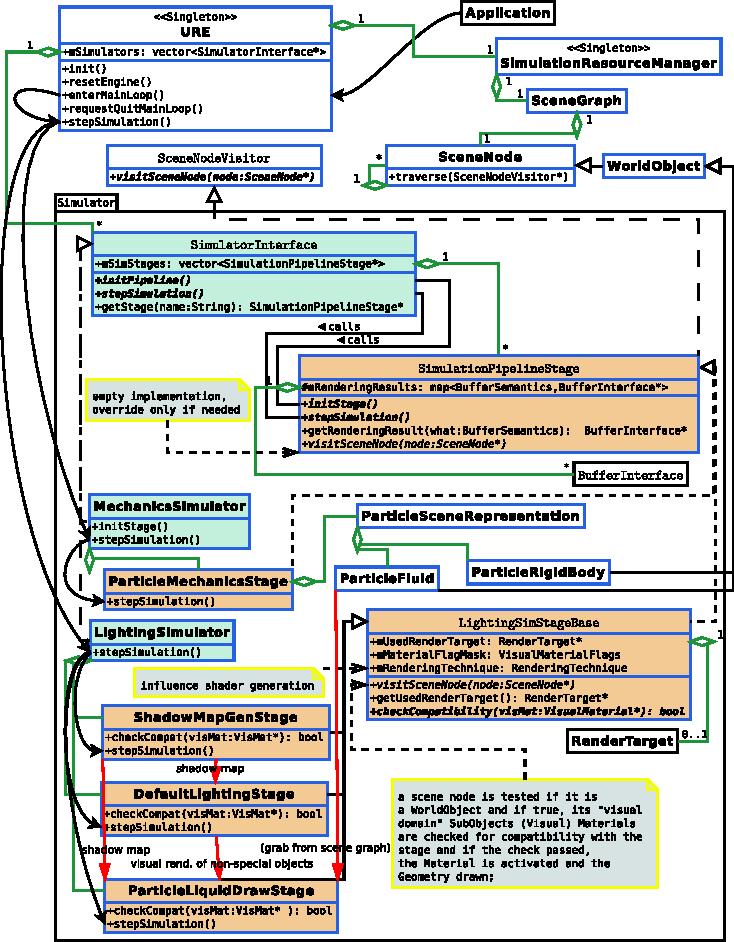
\includegraphics[width=1.15\textwidth]{Detail_Simulator.pdf}
		\caption{Grobes Beispiel von einer Simulation und den zugehörigen Daten-Abhängigkeiten}
		\label{fig:detailSimulator}
	\end{figure}


	Wie bereits erwähnt, soll jede Simulationsdömane einen eigenen Simulator haben, 
	der eine eigene Pipeline an Simulations-Stages verwaltet.
	Es kann theoretisch beliebig viele Simulationsdomänen geben. Momentan sind jedoch nur drei
	über einen \lstinline|enum| definiert: Die visuelle, mechanische und akustische Domäne, wobei
	die akustische Domäne noch nicht in der prototypischen Implementierung vorkommt.
	Abb. \ref{fig:detailSimulator} zeigt grob beispielhaft den Ablauf einer Simulation und die verschiedenen
	Varianten, wie man sich die "`Rendering Results"' anderer Stages beschaffen kann:\\
	Entweder aus der Main Loop der Engine heraus oder von der benutzenden Applikation wird
	\lstinline|URE::stepSimulation()| aufgerufen; Diese Funktion iteriert in fester Reihenfolge über die
	vorhandenen Simulatoren und ruft deren \lstinline|stepSimulation()|-Routine auf; Hierin werden Simulator-
	spezifische Operationen ausgeführt (Framebuffers des Fensters resetten und Haupt-Viewport setzen beim 
	\lstinline|LightingSimulator|, CL/GL-shared Buffers für OpenCL akquirieren beim \lstinline|MechanicsSimulator|...),
	dann über die einzelnen zugehörigen \linebreak
	\lstinline|SimulationPipelineStage|'s iteriert, widerum deren 
	\lstinline|stepSimulation()|-Methode aufgerufen.
	Hier passiert dann das eigentlich \emph{generische Rendering}.
	So verschieden die Algorithmen sind, die in den einzelnen Stages abgearbeitet werden, so verschieden sind auch
	die Möglichkeiten, wie einzelne Stages miteinander Daten austauschen: Der generischste Ansatz ist, sich von einer
	Stage einen Buffer mit einer bestimmten Semantik zu beschaffen, sofern die entsprechende Stage ein solchen
	bereit stellt. Bei Lichtsimulation, die viel mit Texturen und OpenGL-Framebuffer-Objects (FBOs) umgeht,
	bietet sich an, sich das \lstinline|RenderTarget| (die Abtraktion des FBO in \emph{Flewnit}) zu beschaffen,
	um mit dem gesamten RenderTarget weiter zu arbeiten, oder sich einzelne Texturen zu beschaffen.
	Es gibt aber auch die relativ indirekte Methode des Datenaustausches, wie es z.B. zwischen der 
	\lstinline|ParticleMechanicsStage| und der \lstinline|ParticleLiquidDrawStage| der Fall ist: Die Buffer mit dem 		
	physikalischen Attributen sind in der SceneNode-abgeleiteten
	Klasse \lstinline|ParticleFluid| enthalten, so dass die aktualisierten Daten über schlichtes Szenegraphen-Traversieren
	beschafft werden können.\\
	Details zum Ablauf der Simulation(en) werden in Kapitel \ref{sec:simulation} behandelt.




\subsection{Der SimulationResourceManger}
	Diese Singleton-Klasse besitzt und verwaltet die Assets,\linebreak 
	als \lstinline|std::map<String,X*>| für Referenzierung über einen Namen, 
	wobei \lstinline|X| folgende Klassen betrifft: 
	\begin{itemize}
		\item \lstinline|Material|
		\item \lstinline|Geometry|
		\item \lstinline|BufferInterface|
		\item \lstinline|Texture| \footnote{Da \lstinline|Texture| von \lstinline|BufferInterface| erbt, 
		handelt es sich um eine Handle-Sammlung der Untermenge der Texturen aller \lstinline|BufferInterface|s,
		um einen bequemeren Zugriff zu ermöglichen}
		\item \lstinline|InstanceManager|
	\end{itemize}
	Außerdem bestitzt die Klasse den \lstinline|SceneGraph| und stellt einen Handle auf den aktuellen 
	\lstinline|SkyDome| zur Verfügung, so dass alle Objekte ein konsistentes Environment Mapping 
	betreiben können, sofern dies erwünscht ist.

		
\subsection{Das Scene-Paket}		
	Neben dem klassischen Szene-Graphen, der vor allem im Kontext des visuellen Echtzeit-Rendering verwendet wird,
	da er Culling und relative Transformationen ermöglicht, 
	erfordern verschiedene Simulationsdomänen und Repräsentationen der beteiligten Simulations-Objekte
	(z.B. als Dreiecks-Mesh, Komposition von komplexeren Primitiven, Punktwolke oder Voxel-Grid)  ggfs. 
	unterschiedliche Szene-Repräsentationen, damit die spezifischen Anforderungen der Simulation als solchen und der
	Respräsentation der simulierten Objekte optimal erfüllt sind.\\
	Diese Szenen-Repräsentationen unterscheiden sich in der logischen Organisation ihrer Objekte 
	(z.B. Baumstruktur, sortierte oder unsortierte Sammlung, Graph-Struktur, Voxel-Struktur) 
	und in den Meta-Informationen, welche für die einzelnen	Objekte notwendig sind.
	
	Beispielsweise stellt die die effiziente Suche nach räumlich benachbarten Objekten eine wichtige Anforderung
	bei vielen Simulationen (auch bei Lichtsimulation für globale Beleuchtungseffekte) dar.
	Hierfür bieten sich verschiedene Beschleunigungsstrukturen an. Je nach Simulationsdomäne, 
	Objekt-Repräsentation,verwendetem Simulations-Verfahren, verwendeter Hardware und Zielsetzung 
	(Geschwindigkeit, Genauigkeit, Speicherverbrauch...) sind verschiedene Beschleunigungsstrukturen angemessen.
	Somit besteht keine 1:1-Verbindung zwischen Szenen-Repräsentation und Beschleunigungsstruktur.\\
	Beschleunigungsstruktur und Szenen-Repräsentatioen sind somit nur lose gekoppelt.
	Um die verschiedenen Zwecke zu verdeutlichen, stellt Tabelle \ref{tab:sceneRepVsAccStruct} diese gegenüber.

  	%column type with fixed width and centered	
	\newcolumntype{x}[1]{ >{ \centering } p {#1} }
	\begin{table}	 	
	 	\begin{tabular}
  		{ x{0.33\textwidth} | x{0.33\textwidth} | x{0.33\textwidth} | }	
  					\cline{2-3}
  					& Szenen-Repräsentation & Beschleunigungsstruktur
  					\tabularnewline\cline{1-3}
  		\multicolumn{1}{ |c| }{
  			Organisation der Elemente
  		}			&	
  						logisch für Zugriff auf Ebene der Anwendungslogik
  					&  
						räumlich für effizienten Zugriff durch einen Simulations-Algorithmus
  			 		\tabularnewline\cline{1-3}
   		\multicolumn{1}{ |c| }{
  			Zweck von Meta-Informationen
  		}			&
  						verschieden, je nach Repräsentation und Typ der Simulations-Objekte	
  					&	
  						(sofern vorhanden) unterschliedlich für verschiedene Algorithmen, z.b.
 						effiziente Traversierung und/oder Nachbarschaftssuche
  					\tabularnewline\cline{1-3}	  	  	
	  	\end{tabular}	  	
  		\caption{Gegenüberstellung der Zwecke einer generischen Szenen-Repräsentation und einer Beschleunigungsstruktur}
  		\label{tab:sceneRepVsAccStruct}
	\end{table}	
	
	Es gibt also zwei Basis-Klassen, wie in Abb. \ref{fig:ClassDiagOverview2} zu sehen ist:
	\lstinline|SceneRepresentation| und \lstinline|AccelerationStructure|.
	\lstinline|AccelerationStructure| erbt von \lstinline|WorldObject|(siehe Abschnitt \ref{sec:worldObject}),
	um optional Debug-Draw-Funktionalität bereit zu stellen.
	Ansonsten handelt es sich schlicht um abstrakte Basis-Klassen ohne weitere Funktionalität.
	
	Für das gesamte System über den \lstinline|SimulationResourceManger| verfügbar ist der
	\lstinline|SceneGraph|. Dieser enthält die Wurzel-\lstinline|SceneNode|, welche beliebig viele Kinder derselben
	Klasse haben kann. Somit wird eine Baumstruktur gebildet.\\
	Die SceneNode bildet die Basis-Klasse des \lstinline|WorldObject| (siehe Abschnitt \ref{sec:worldObject}).
	
	Es ist ein Mechanismus konzipiert, sowohl Kinder als auch Vorfahr über Änderungen der eigenen Transformation
	und/oder Bounding Box zu informieren, so dass ggfs. globale Transformationen akkumuliert werden können und/oder
	die Bounding Box für den eigenen Unterbaum ermittelt, die für Culling-Berechnungen verwendet werden kann.
	Noch ist dieses Feature nicht in Nutzung und seine Implementation unvollständig und ungetestet,
	daher wird auf weitere Details	verzichtet.
	
	Die klassischen Operationen (Einfügen, Aushängen, rekursives Suchen im Unterbaum nach Namen, Node bewegen,
	Transformationen akkumulieren) sind jedoch implementiert. Es sei an die enge Kopplung dieser Klasse an
	\lstinline|AmendedTransform| (s. Abschnitt \ref{{sec:AmendedTransform}}) erinnert.
	
	Der Scenegraph kann nach dem Visitor- Design Pattern traversiert werden. Z.B. erbt 
	\lstinline|SimulationPipelineStage| von \lstinline|SceneNodeVisitor|, so dass bei Bedarf eine Pipeline-Stage
	nur \lstinline|virtual void visitSceneNode(SceneNode* node)| implementieren muss, um Operationen auf oder mit
	den Objekten des Szenegraphen auszuführen.
	Momentan "`besitzt"' die \lstinline|SceneNode|-Klasse seine Kinder, was den Vorteil hat, dass die Nodes nicht woanders
	verwaltet werden müssen, aber den Nachteil, dass ausgehängte Scene Nodes nicht automatisch beim Reset der Engine
	gelöscht werden. Sollte sich dies später als Problem herausstellen, könnte man die Scene Nodes auch vom
	\lstinline|SimulationResourceManger| verwalten lassen.
	Auch empfiehlt sich langfristig die Möglichkeit zur Erschaffung und Verwaltung mehrerer Szenegraphen.
	Aus Zeitgründen habe ich es jedoch erstmal bei dieser rudimentären Implementation belassen.
	
	Intern verwaltet die \lstinline|ParticleMechanicsStage|, die \lstinline|SimulationPipelineStage|,
	die im \lstinline|MechanicsSimulator| für die partikelbasierte Simulation zuständig ist, 
	eine \lstinline|ParticleSceneRepresentation|. Diese verwaltet 
	\begin{itemize}
		\item die "`makroskopischen Objekte"', die an dieser Simulation teilnehmen,
		namentlich (allesamt von \lstinline|WorldObject| abgeleitete) 
		partikelbasierte Fluide, partikel-repräsentierte Rigid Bodies und statische Kollisions-Meshes
		\footnote{diese müssen in einem bestimmten Format vorliegen}
		\item die einzelnen Attribute-Buffers der Partikel
			(Position, Dichte, Geschwindigkeit, Beschleunigung usw.)
		\item Buffers mit Meta-Informationen der "`makroskopischen Objekte"', die an OpenCL-Kernels übergeben werden
	\end{itemize}
	Ferner stellt die Klasse Factory-Methoden für die makroskopischen Objekte bereit, da diese direkt mit den
	Partikel-Buffern assoziiert sind, sich also alle beteiligten Objekte die Buffers teilen müssen. Die korrekte
	Delegierung der Offsets und Sicherstellung der richtigen Größen wird so übernommen.\\
	Die \lstinline|ParticleMechanicsStage| nutzt außerdem ein \lstinline|UniformGrid| für die Simulation.
	Details hierzu werden im Verlauf des Kapitels \ref{sec:mechanicalDomain} beschreiben.
	
	


\subsection{Das WorldObject}
	\label{sec:worldObject}
	Das \lstinline|WorldObject| stellt die abstrakte Basisklasse für sämtliche Objekte dar, mit denen eine oder mehrere 
	Simulationen durchgeführt werden sollen\footnote{Und sei es nur Debug Drawing; Selbst dies kann als eine 
	rudimentäre Form von Lichtsimulation aufgefasst werden.}. Sie erbt von \lstinline|SceneNode|. Damit ist sie bequem 
	in den Szenegraphen integrierbar und hat außerdem schon seinen Transformations-Membervariable.
	
	Bei dieser Klasse zeigt sich erstmals die angestrebte Symmetrie zwischen sen Simulationsdömanen: 
	Für jede Simulationsdomäne
	gibt es eine (möglicherweise leere) Liste an \lstinline|SubObject|'s. Das \lstinline|SubObject| 
	stellt eine Abstraktion dessen dar, was in einer klassischen Graphik-Engine ein "`SubMesh"' oder
	in einer klassischen Physik-Engine eine Komponente einer "`(Compound) Collision Shape"' sein könnte.\\
	Ein \lstinline|SubObject| hat immer einen Pointer auf genau ein \lstinline|Material|, 
	eine \lstinline|Geometry|  und für Backtracking-Zwecke auf sein besitzendes	\lstinline|WorldObject|.
	Wie der Backtracking-Pointer andeutet, besitzt das ein \lstinline|WorldObject| jedes seiner \lstinline|SubObject|s.
	Die vom \lstinline|SubObject| genutzte Geometrie und Materialien können jedoch --sofern sinnvoll -- von beliebig
	vielen \lstinline|SubObject|s gemeinsam genutzt werden.
	
	Es sind verschiedenste Ableitungen von \lstinline|WorldObject| denkbar, z.B. 
	(standard/particle based/voxel based) Rigid Body, Soft Body, rein visuelles Objekt,  
	Kamera,Lichtquelle, Debug-Draw-Objekte, Cloth, Hair, oder (particle based/voxel based) Fluid.
	
	Welche Objekte im Szenegraph für die Nutzung in einer Simulations-Stage in Frage kommen, lässt sich entweder
	über eine Vorfilterung bei Objekt-Erstellung (Factory-Pattern oder automatische Registierung bei einer 
	Manager-Klasse im Konstruktor), oder über \lstinline|dynamic_cast<>()|'s und anschließendes Auslesen von spezifischer
	Meta-Information ermitteln, oder aber durch "`property flags"', also Bit-Flags, die Features einer Scene Node andeuten.
	Welche dieser Methoden langfristig die robusteste, flexibelste und eleganteste ist,
	vermag ich noch nicht zu sagen. Da Typ-Informationen über \lstinline|enum|s 
	(als Bitflags oder "`normale"' Aufzählungstypen)
	eine gewisse Redundanz hat ggü. der dynamischen Typ-Information, die C++ bereit stellt, und außerdem eine weitere
	Fehlerquelle für den Programmierer darstellt, sind die Bitflags nicht erste Wahl. Außerdem schränkt die explizite 
	Auflistung von Features womöglich die Erweiterbarkeit des Systems ohne komplette Neu-Kompilierung ein.
	Andererseits machen sie Programme vielleicht lesbarer, indem bestimmte Kategorien/Features explizit aufgelistet 
	(und im Falle von Bitflags beliebig kombinierbar) sind, 
	und nicht implizit in C++-Typinformationen codiert sind.
	Ich verwende Aufzählungstypen intensiv in \emph{Flewnit}. Nicht immer sind diese für die Programmlogik nötig.
	Sie halfen mir jedoch zur Strukturierung und Ideen-Sammlung. Letztere ist wichtig, da bei einem Softwaresystem,
	welches generische Verwendbarkeit anstrebt, schon weit vor Implementierung konkreter Klassen die Struktur der
	Basisklassen anhand von abstrahierten (erwarteten) gemeinsamen Features der möglichen abgeleiteten Klassen
	möglichst exakt bestimmt werden sollte. Je weiter oben in der Klassenhierarchie Design-Fehler auftauchen, desto
	aufwändiger droht das spätere Refactoring zu werden.

%	Die Entscheidung, dass \lstinline|WorldObject| abstrakt sein soll, wurde getroffen, damit keine Funktionalität,
%	die zunächst generisch erscheint, sich aber später als doch nicht allgemein auf alle konkreten 
%	\lstinline|WorldObjects| anwendbar herausstellt, diese Basisklasse verunreinigt. 
%	Es sind so viele verschiedenste Ableitungen denkbar (Rigid Body, Soft Body, rein visuelles Objekt, Kamera,
%	Lichtquelle, Debug-Draw-Objekte, Cloth, Hair, Fluid...)	
  
 
\subsection{Material}  

	Der Begriff "`Material'", der sich in der Computergraphik eingebürgert hat als Beschreibung von visuellen Eigenschaften
	einer Oberfläche, erscheint mir prädestiniert, sich in seiner Bedeutung in einem alltäglichen,
	nicht computergraphischen Kontext wieder anzunähern:
	das \emph{Material} in \emph{Flewnit} steht für "`sämtliche Eigenschaften von Materie 
	außer ihrer geometrischen Form und internen Repräsentation dieser"'.

	\begin{figure}[!h]
		\centering
	   	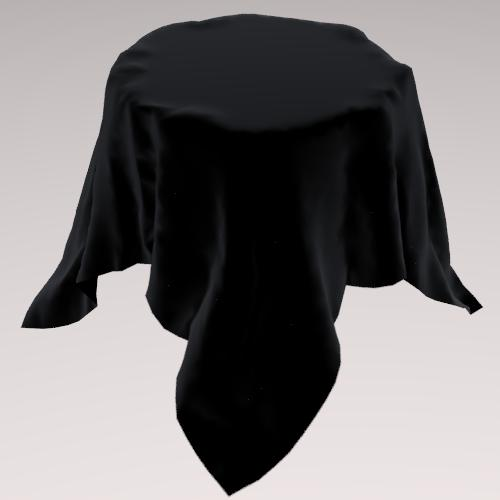
\includegraphics[width=0.3\textwidth]{velvetBlack1.jpg}
		\caption{ Der Begriff \emph{Material} mit einer physikalisch orientierten Bedeutung:
			sämtliche Eigenschaften von Materie	außer ihrer geometrischen Form.
			(Bild entnommen aus \cite{microfacet})
		}
		\label{fig:material}
	\end{figure}
	
	Würden wir über die entsprechende Rechenleistung verfügen und als Programmierer das physikalische Know-How
	besitzen (z.b. über Maxwell'sche Gleichungen), bräuchte man dieses Konzept gar nicht weiter zu konkretisieren,
	und könnte sämtliches Verhalten von Simulations-Objekten durch subatomare Material-Eigenschaften modellieren.
	Dies wäre eine "wirkliche" Vereinheitlichung der bestehenden Engine-Konzepte, die unserer Realität Rechnung trüge.
	Da wir jedoch realistisch (im Sinne der Machbarkeit) bleiben wollen jetzt und heute Echtzeit-Fähigkeit,
	auch auf Kosten von physikalischer Korrektheit/Genauigkeit anstreben, sind Domänen-spezifische Konkretisierungen des
	Material-Konzeptes notwendig, und wie so viele andere Klassen in diesem System wird die 
	\lstinline|Material|-Klasse zur abstrakten Oberklasse.
	Bei einem \lstinline|SubObject|, welches der visuellen Simulationsdömane angehört, wird implizit erwartet,
	dass das genutzte \lstinline|Material| ein \lstinline|VisualMaterial| ist 
	(mit Texturen, Shader, und verscheiedenen Meta-Informationen, um das visuelle Rendering zu delegieren,
	siehe Abschnitt \ref{sec:visualMaterial}), 
	und in der mechanischen Domäne muss es ein \lstinline|MechanicalMaterial|(mit Eigenschaften wie Masse, Reibung, 	
	Elastizität etc.) sein. Diese domänenspezifischen Material-Typen können oder müssen (je nach Typ des nutzenden
	\lstinline|WorldObject|s) noch weiter abgeleitet sein.
	
	Einen etwas schalen Beigeschmack haben die Routinen:
	\begin{lstlisting}
virtual void activate(
		SimulationPipelineStage* currentStage,
		SubObject* currentUsingSuboject) throw(SimulatorException){}
//undoing stuff, like re-enable depth test etc.
virtual void deactivate(SimulationPipelineStage* currentStage,
		SubObject* currentUsingSuboject) throw(SimulatorException){}
	\end{lstlisting}
	Sie sind dem Statemachine-basierten visuellen Rendering mit OpenGL zu verdanken und müssen daher von den
	\lstinline|VisualMaterial|-Klassen implementiert werden. Um der Möglichkeit Rechnung zu tragen, dass
	ähnlich State-basierte Mechanismen an anderer Stelle als beim OpenGL-Rendering vorkommen sollten, sind diese
	Routinen in die Oberklasse gelangt.

	

    	
\subsection{Die Buffer-Abstraktion}  
	%Abschnitt ausgelagert weil er zu groß wurde!
	\label{sec:architecture:BufferAbstraction} 	

	Logischerweise müsste nun eigentlich 
	-- der Top-Down-Präsentation der einzelnen Pakete und Klassen entsprechend --
	die \lstinline|Geometry|-Klasse vorgestellt werden. Um letztere Klasse jedoch besser zu verstehen,
	ist die Kenntnis der Buffer-Abstraktion vorteilhaft. Die \lstinline|Geometry| wird in \ref{sec:geometry} beschrieben.
	
	Wie auf Seite \pageref{overview:bufferAbstraction} erwähnt, abstrahiert die \lstinline|BufferInterface|-Klasse
	sämtliche Buffer-bezogene Funktionalität, namentlich für Host-Buffer, OpenCL-Buffer, 
	verschiedene OpenGL-Buffertypen und letztendlich verschiedene Texturtypen (eine Teilmenge davon ist OpenCL-interop-
	kompatibel bzw als reine OpenCL-Textur erschaffbar).
	Es ergibt sich ein wahrer Moloch, der für eine relativ einheitliche Handhabung zu abstrahieren ist: 
	
	\begin{itemize}
		\item verschiedene APIs (OpenGL C-Api "`vs."' OpenCL C++-API)
		\item verschiedene Verwendungen und Verfügbarkeiten schon allein von non-Textur-Buffern 
			(generisch, Vertex Index/Vertex Attribute Buffer, Uniform Buffer, Render Buffer),
			siehe Tabelle \ref{tab:bufferSupportInContexts}
		\item verschiedene OpenGL-Texturtypen mit nur bedingt kombinierbaren und nur teilweise zu OpenCL kompatiblen 
			erweiterten  Features, siehe Tabelle \ref{tab:textureTypes} 
			%(Tiefentextur ja/nein, MipMapping ja/nein, Textur-Array ja/nein, Multisample-Texture ja/nein, 
			%Rectangle Texture ja/nein, Cube Map ja/nein)
		\item verschiedene Datenformat/Channel-Layout-Deskriptoren, siehe Listing \ref{listing:BufferElementInfo}
	\end{itemize}	
	
	Es hat schon sehr viel Zeit gekostet, sich aus den Spezifikations-Dokumenten 
	(\cite{openGL_4_1_Spec}, \cite{openCL_1_0_Spec}) die möglichen Permutationen, Zusammenhänge, Entsprechungen
	und unterstützten Operationen zu erarbeiten 
	(siehe Tabellen \ref{tab:channelLayoutAndTypes} und \ref{tab:textureTypes}).
	
	Die Ergebnisse dieser Tabellen flossen in die Entscheidung ein, welche konkreten Buffer-
	und Textur-Klassen mit welchen  verfügbaren Features durch Ableitung vom
	\lstinline|BufferInterface| implementiert wurden. Die Konstruktor-Parameter sollten
	so spezifisch zugeschnitten sein, dass der Benutzer der Klassen möglichst wenig invalide
	Kombinationen angeben kann. Außerdem sollte er sich nicht um all die Makros
	wie \lstinline|GL_RGBA32UI| bzw \lstinline|CL_RGBA| und \lstinline|CL_UNSIGNED_INT32|
	kümmern müssen 
	\footnote{Was in OpenCL getrennt ist und somit "`nur"' 
		4 Channeltypen \emph{+} 3 Bitgrößen * (3 non-normalized + 2 normalized)= theoretisch 19 makros ergibt,
		braucht bei OpenGL
			4 Channeltypen \emph{*} 3 Bitgrößen * (3 non-normalized + 2 normalized)= theoretisch 60 makros;
			Erstens stört die Asymmetrie, zweitens das "`Zusammenklatschen"' eigentlich unabhängiger Parameter in ein 
			Makro}. 
	Es soll ein Buffer mit einem einzigen Konstruktor-Call völlständig definiert,
	falls erwünscht auf dem Host-Memory und -- sofern unterstützt --
	in den gewünschten API-Contexten allokiert bzw registiert werden.
	
	Hierfür mussten einige \lstinline|enum|s und Meta-Info-Klassen/Structures definiert werden:
	\begin{description}
		
		\item[enum Type] 
		Beschreibt String-, boolsche, Skalar-, Vektor- und Matrix-Datentypen mit verschiedener 
		Genauigkeit. Findet in \emph{Flewnit} u.a. auch beim Config-Parsen Verwendung.
		
		%--------------------------------------------------------------------------------------------
		\item[enum ContextType und ContextTypeFlags] 
		Mithilfe dieser Datentypen lässt sich spezifizieren, in welchem 
		Kontexten (Host, OpenGL, OpenCL) man einen Buffer erstellt/allokiert/registriert haben will.
		
		%--------------------------------------------------------------------------------------------
		\item[enum BufferSemantics] 
		Eine sehr wichtige Auflistung konkreter Verwendungszwecke des Buffers,
		siehe Listing \ref{listing:BufferSemantics} im Anhang \ref{append:bufferListings}.
		Dieser Aufzählungstyp ist eine große Erleichterung beim Hantieren mit OpenGL Vertex Buffer Objects (VBO's) 
		\footnote{abstrahiert von \lstinline|Flewnit::VertexBasedGeometry|, s. \ref{sec:geometry} }
		und Frame Buffer Objects (FBO's) 
		\footnote{abstrahiert von \lstinline|Flewnit::RenderTarget|}, 
		da hier zur Assoziation von VBO-Vertex Attribute Buffern mit Input-Variablen im Vertex Shader
		bzw and FBO gehängte Texturen mit Output-Variablen im Fragment Shader
		ein Index angegeben werden muss. 
		Wenn wir als Index die numerische Entsprechung der Buffer-Semantik verwenden, 
		ist nicht nur die Lesbarkeit des Codes erhöht, es ist auch automatisch sichergestellt, 
		dass Indizes keine Konflikte versursachen!
		
		%--------------------------------------------------------------------------------------------
		\item[enum GPU\_DataType] Listet nur die von der GPU / OpenGL nativ unterstützten Datentypen auf, ohne
		Präzisions- und Normalisierungs-Information:
		\begin{lstlisting}		
enum GPU_DataType
{
	GPU_DATA_TYPE_FLOAT,
	GPU_DATA_TYPE_INT,
	GPU_DATA_TYPE_UINT
};
		\end{lstlisting}
		
		%--------------------------------------------------------------------------------------------
		\item[enum GLBufferType]
		Listet die vom Buffer-Interface abstrahierten OpenGL-non-Textur-Buffertypen auf. 
		Aus Zeitgründen und Erwartung, dass sie außerhalb der \lstinline|RenderTarget|-Klasse nicht benötigt werden,
		werden z.B. Render Buffers nicht abstrahiert.
		\begin{lstlisting}		
enum GLBufferType
{
	NO_GL_BUFFER_TYPE,
	VERTEX_ATTRIBUTE_BUFFER_TYPE,
	VERTEX_INDEX_BUFFER_TYPE,
	UNIFORM_BUFFER_TYPE 
};
		\end{lstlisting}	
	
		%--------------------------------------------------------------------------------------------
		\item[struct BufferElementInfo] 
		Beschreibt -- sofern erwünscht bzw nötig -- das Channel-Layout,die Datentypen, die Bit-Genauigkeit
		und die etwaige Normalisierung eines Buffers mit Channels, 
		z.B. einer Textur oder einem Vertex Attribute Buffer,
		siehe Listing \ref{listing:BufferElementInfo} im Anhang \ref{append:bufferListings}.
		Auf diese Weise spart man sich die verschiedenen "zusammengesklatschten", asymmetrischen GL/CL-Makros;
		Die Structure validiert ihre Daten. Diese werden später für die internen CL/GL-API-Aufrufe in die
		entsprechenden CL/GL-Makros transformiert,
		siehe Listing \ref{listing:BufferElementInfoToCLGL} im Anhang \ref{append:bufferListings}.
		
		%--------------------------------------------------------------------------------------------
		\item[struct GLImageFormat]
		OpenCL definiert folgende Structure:
		
		\begin{lstlisting}		
typedef struct _cl_image_format {
    cl_channel_order        image_channel_order;
    cl_channel_type         image_channel_data_type;
} cl_image_format;	
		\end{lstlisting}
		
		Um das interne Handling der CL/GL-Makros etwas symmetrischer zu machen (man verliert leicht den Überblick),
		habe ich ein ähnliches Makro definiert, welches aufgrund der Kommentare im Anhang  \ref{append:bufferListings},
		Listing \ref{listing:GLImageFormat} zu finden ist.\footnote{Die Kommentare geben weiteren Aufschluss über 
		die Asymmetrie der einzelnen APIs: obwohl sie beide von der Khronos Group spezifiziert wurden und explizit 	
		Interoperabilität ermöglichen, stiften viele mehr oder minder kleine Asymmetrien Verwirrung (zumindest bei mir);
		Diese Umstände trugen zu der Entscheidung bei, das \lstinline|BufferInterface| zu entwickeln, trotz des
		erheblichen Zeitaufwands.}
		
		
		\item[class BufferInfo]
		Dies ist die Klasse, die sowohl als "`Construction Info"' den Konstruktor-Code delegiert, als auch für 
		den benutzer später Meta-Information bereitstellt.
		Es sei hier nur der Standard-Konstruktor angegeben:
		
		\begin{lstlisting}	
explicit BufferInfo(String name,
	ContextTypeFlags usageContexts,
	BufferSemantics bufferSemantics,
	Type elementType,
	cl_GLuint numElements,
	const BufferElementInfo& elementInfo,
	GLBufferType glBufferType = NO_GL_BUFFER_TYPE,
	ContextType mappedToCPUContext = NO_CONTEXT_TYPE);
		\end{lstlisting}
		
		Ich muss zugeben, dass \lstinline|elementType| und \lstinline|elementInfo| redundant sind, außerdem diese 
		beiden Parameter eigentlich bei generischen Buffern, wo die Typ-Information zumindest für die GPU Computing APIs
		keine Rolle spielt, fehl am Platze sind. Mangelndem Überblick in der Anfangsphase der Implementierung
		über die Verschiedenen Arten, Buffers in CL und GL zu nutzen, sind diese Design Flaws zuzuschreiben.
		Ein Refactoring mit besser speziell zugeschnittenen Konstruktoren ist geplant.
		zu nutzen
	
	\item[class TextureInfo]
		So wie \lstinline|Texture| von \lstinline|BufferInterface| erbt, erbt auch 
		\lstinline|TextureInfo| von \lstinline|BufferInfo|. Sie stellt die gleiche Funktionalität für
		die (abstrakte) \lstinline|Texture|-Klasse dar wie \lstinline|BufferInfo| für \lstinline|BufferInterface|.
		Ein Unterschied besthet jedoch darin, dass \lstinline|TextureInfo| eigentlich nur dazu dient, 
		die kombinierte Information aus den Parametern der "`eingeschränkten"' Konstruktoren 
		der konkreten Textur-Klassen (\lstinline|Texture2D| etc.) und der inhärent klassenspezifischen
		Eigenschaften an die \lstinline|Texture|-Oberklasse zu übergeben. Damit hat \lstinline|TextureInfo|
		eher eine Textur-interne Funktion bei der Konstruktion. Das tut jedoch seiner Funktion als späterer
		Meta-Daten-Lieferant keinen Abbruch.
		Auch hier reicht der Standard-Konstruktor für eine Idee dieser Klasse:
		 
		\begin{lstlisting}	
explicit TextureInfo(
	const BufferInfo& buffi,
	cl_GLuint dimensionality,
	Vector3Dui dimensionExtends,
	GLenum textureTarget,
	bool isDepthTexture = false,
	bool isMipMapped = false,
	bool isRectangleTex = false,
	bool isCubeTex = false,
	GLint numMultiSamples = 1,
	GLint numArrayLayers = 1
	);
		\end{lstlisting}			
			
	\end{description}	

 	
 	\begin{table}[!h]
  		\begin{tabular}
  		{
  		 l  l | c | c | c |
  		}
																	\cline{3-5}
  									&								&	\multicolumn{3}{ c | }{Context} \\ 
  																	\cline{3-5}
									&								& 	Host 	& 	OpenGL 	& 	OpenCL	\\
    	\noalign{\hrule}								
    	\multicolumn{1}{|c|}{
    		generic Buffer
    	}							& 								
    		&	{\color{green}\checkmark} 	&	{\color{red}x}		& 	{\color{green}\checkmark}	\\ 
    	
    	\noalign{\hrule}								
    	\multicolumn{1}{|c|}{
    		\multirow{4}{*}{OpenGL Buffers}
    	}							& Vertex Attribute Buffer		
    		&	{\color{orange}o} 	&	{\color{green}\checkmark}		& 	{\color{orange}o}	\\  
    								\cline{3-5}
    	\multicolumn{1}{|c|}{}		& Vertex Index Buffer			
    		&	{\color{orange}o} 	&	{\color{green}\checkmark}		& 	{\color{orange}o}	\\  
    								\cline{3-5}
    	\multicolumn{1}{|c|}{}		& Uniform Buffer
    		&	{\color{orange}o} 	&	{\color{green}\checkmark}		& 	{\color{orange}o}	\\ 
    								\cline{3-5} 
    	\multicolumn{1}{|c|}{}		& Render Buffer					
    		&	{\color{red}x} 	&	{\color{green}\checkmark}		& 	{\color{green}\checkmark}	\\ 
    
   		\noalign{\hrule}								
   		\multicolumn{1}{|c|}{
    		\multirow{4}{*}{Textures} 
   		}							& 1D Texture					
   			&	{\color{orange}o} 	&	{\color{green}\checkmark}		& 	{\color{red}x}	\\ 
    								\cline{3-5}
		\multicolumn{1}{|c|}{}		& 2D Texture				
			&	{\color{orange}o} 	&	{\color{green}\checkmark}		& 	{\color{green}\checkmark}	\\ 
									\cline{3-5}
		\multicolumn{1}{|c|}{}		& 3D Texture		
			&	{\color{orange}o} 	&	{\color{green}\checkmark}		& 	{\color{green}\checkmark}	\\ 
									\cline{3-5}
		\multicolumn{1}{|c|}{}		& Special Texture				
			&	{\color{orange}?} 	&	{\color{green}\checkmark}		& 	{\color{orange}?}	\\ 


    	\noalign{\hrule}
     
     	
  		\end{tabular}	
  	
  		\caption{		
  			Verschiedene Buffertypen und ihre Verfügbarkeit in verschiedenen Kontexten \\	
  			Legende: \\
			{\color{green}\checkmark}	$\rightarrow$ nativ unterstützt;
			{\color{orange}o}	$\rightarrow$ kompatibel;
			{\color{red}x}	$\rightarrow$ nicht unterstützt;	\\
			{\color{orange}?}	$\rightarrow$ Unterstützung abhängig von weiteren Parametern, 
								s. Tabelle \ref{tab:textureTypes};	
		}
		\label{tab:bufferSupportInContexts}
  	\end{table}
  	
  	
  	\begin{table}[!h]
  		\begin{tabular}
  		{
  			|l|c|c|c|c|c|
  		}
		\noalign{\hrule}						
  						&	CL interop	&	MipMap	& Depth	&	Array	&	Rectangle	\\
  		\noalign{\hrule}						
  		Texture1D		& {\color{red}x} & {\color{green}\checkmark} & {\color{red}x}
  						& {\color{green}\checkmark} & {\color{red}x} \\
		\noalign{\hrule}						
  		Texture2D		& {\color{green}\checkmark} & {\color{green}\checkmark} & {\color{green}\checkmark}  
  						& {\color{green}\checkmark} & {\color{green}\checkmark} \\
  		\noalign{\hrule}						
  		Texture2DCube 	& {\color{yellow}o} & {\color{green}\checkmark}  & {\color{green}\checkmark}
  						& {\color{orange}o} & {\color{red}x} \\
  		\noalign{\hrule}						
  		Texture2DMultiSample& {\color{red}x} & {\color{red}x}  & {\color{red}x} 
  						& {\color{green}\checkmark} & {\color{red}x} \\	
  		\noalign{\hrule}						
  		Texture3D		& {\color{green}\checkmark} & {\color{green}\checkmark}  & {\color{red}x} 
  						& {\color{red}x} & {\color{red}x} \\
  		\noalign{\hrule}						
  		\end{tabular}
  		
  		\caption{Verschiedene Texturtypen und ihre Kompatibiltät zu bestimmten Features \\	
  			Legende: \\
			{\color{green}\checkmark}	$\rightarrow$ unterstützt;
			{\color{yellow}o}	$\rightarrow$ In OpenCL unterstützt, aber nicht vom Framework;
			{\color{orange}o}	$\rightarrow$ nur in OpenGL 4 unterstützt,
								daher wegen Kompat. zu GL 3 nicht vom Framework unterstützt;
			{\color{red}x}	$\rightarrow$ nicht unterstützt;
		}
  		\label{tab:textureTypes}
	\end{table}
	
	Es sei bemerkt, dass die Tiefen-Texturen sich abgesehen von den automatisch bestimmten
	entsprechenden OpenGL-Makros in ihrer Implementation nur geringfügig von ihren "`Farbtextur"'-
	Oberklassen unterscheiden, nämlich in der Implementation der 
	\lstinline|virtual void setupDefaultSamplerParameters()=0;|-Methode, die in \lstinline|Texture| definiert ist.
	Hier z.B. der Compare-Mode und die Compare-Function für korrekten Lookup solcher Texturen als Shadow Map
	über einen	Shadow-Sampler in GLSL.
	
	Man darf sich fragen, warum ich jede noch so sonderbar anmutende Spezial-Textur unterstützen will. Dies
	hat den Grund, dass ich langfristig etliche Rendering Features unterstützen will, welche die meisten dieser 	
	Spezialtexturen benötigen, und die verbleibenden paar ungenutzten Texturen noch zur Vollständigkeit mit zu 
	implementieren, verursacht dank Vererbung nur einen minimalen Mehraufwand:
	\begin{enumerate}
		\item Layered Rendering in \lstinline|Texture2DDepthCube| zur Generierung von Point Light Shadow Maps
		in nur einem Rendering Pass
		\item Layered Rendering in \lstinline|Texture2DCube| zur Generierung von dynamischen Environment Maps
		\item  Layered Rendering in \lstinline|Texture2DDepthArray| zur Generierung von vielen Spot Light Shadow Maps
		in nur einem Rendering Pass
		\item Deferred Shading mit Multisampling: Benötigt \lstinline|Texture2DMultiSample|-G-Buffers
	\end{enumerate}
	Zu weiten Teilen sind der Shadercode und die nötigen Framework-Klassen schon für diese Features implementiert,
	es muss "`nur"' noch einiges ergänzt und aufgeräumt, alles zusammengefügt und debuggt werden. 
	Da dieses "`Nur"' wirklich äußerst ironisch gemeint ist, habe ich gar nicht erst versucht, 
	die Implementierung dieser Features zu beenden. Es muss vorerst reichen,
	dass sie konzeptionell in der Framework-Struktur angelegt sind.
	
	
	%------------------------------------------------------------------------------------------
	
	Alle Operationen auf den Buffern/Texturen werden dann über das \lstinline|BufferInterface|
	getätigt. Fast sämtlicher Kontrollfluss (Synchronisation,Validierung, Auswahl des richtigen Kontextes etc.)
	befindet sich in der Implementation	der (wohlgemerkt großteils \emph{nicht} virtuellen) 
	Methoden von \lstinline|BufferInterface|. 
	Nur die finale Bürde der verschiedenen API-Calls als Ergebnis des vorangegangenen Kontrollflusses
	wird von \lstinline|protected| virtuellen Funktionen der abgeleiteten Klassen übernommen, wie im folgenden 	
	Unterabschnitt beschrieben.
	
	\subsubsection{Die API-bezogenen internen Buffer-Operationen}
	Zur Vermeidung von Boilerplate-Code sind die Signaturen für die GPU Computing API-bezogenen 
	Buffer-Operationen ausgelagert in eine Datei namens "`BufferVirtualSignatures.h"'.
	Um sowohl in der abstrakten Basisklasse als auch in den abgeleiteten Klassen included werden zu können,
	lässt sich die Abstraktheit der Definitionen über das Makro \lstinline|FLEWNIT_PURE_VIRTUAL| steuern:
		
	\begin{lstlisting}[caption={API- und Buffertyp-abhängige Operationen auf Buffern -- Definitionen},
					   label=listing:bufferOpDefs]	
#ifdef FLEWNIT_PURE_VIRTUAL
#	define PURENESS_TAG =0
#else
#	define PURENESS_TAG
#endif

	virtual void generateGL()	throw(BufferException)	PURENESS_TAG;
	virtual void generateCL()		throw(BufferException)	PURENESS_TAG;
	virtual void generateCLGL()		throw(BufferException)	PURENESS_TAG;

	//there is no pendant to bind() in OpenCL, as the API needs no buffer binding mechanism;
	//instead, buffers are passed as arguments to kernels
	virtual void bindGL()			throw(BufferException)	PURENESS_TAG;
	//there is no pendant to alloc() in OpenCL, as Buffer generation and allocation are coupled within
	//the same API call
	virtual void allocGL()			throw(BufferException)	PURENESS_TAG;

	virtual void writeGL(const void* data)throw(BufferException)	PURENESS_TAG;
	virtual void writeCL(const void* data)throw(BufferException)	PURENESS_TAG;
	virtual void readGL(void* data)		throw(BufferException)	PURENESS_TAG;
	virtual void readCL(void* data)		throw(BufferException)	PURENESS_TAG;
	virtual void copyGLFrom(GraphicsBufferHandle bufferToCopyContentsFrom)throw(BufferException)	PURENESS_TAG;
	virtual void copyCLFrom(ComputeBufferHandle & bufferToCopyContentsFrom)throw(BufferException)	PURENESS_TAG;
	//because the C++ Wrapper for OpenCL is used, deletion takes place automatically when th cl::Buffer is destroyed
	virtual void freeGL()			throw(BufferException)	PURENESS_TAG;
	
//	//not implemented yet as not needed at the moment: mapping routines:
//	virtual void* mapGLToHost()throw(BufferException)	FLEWNIT_SIGNATURE_PURENESS_TAG;
//	virtual void* mapCLToHost()throw(BufferException)	FLEWNIT_SIGNATURE_PURENESS_TAG;
//	virtual void* unmapGL()throw(BufferException)	FLEWNIT_SIGNATURE_PURENESS_TAG;
//	virtual void* unmapCL()throw(BufferException)	FLEWNIT_SIGNATURE_PURENESS_TAG;

#undef PURENESS_TAG
	\end{lstlisting}
	
	So included \lstinline|BufferInterface| diese Datei innerhalb ihrer Klassendefinition über
	\begin{lstlisting}
#	define FLEWNIT_PURE_VIRTUAL
#	include "BufferVirtualSignatures.h"
#	undef FLEWNIT_PURE_VIRTUAL
	\end{lstlisting},
	
	die anderen Klassen definieren das Makro nicht vor dem Includen.\\
	
	In Anhang \ref{append:bufferListings} sind exemplarisch Implementationen dieser Funktionen 
	gelistet, einerseits die der konkreten \lstinline|Buffer|-Klasse (Listing \ref{listing:bufferOpImpls_Buffer}),
	 die alle non-Textur-Buffer zusammengefasst abstrahiert, 
	andererseits die der konkreten \lstinline|Texture2D|-Klasse 
	(Listing \ref{listing:bufferOpImpls_Texture} und \ref{listing:bufferOpImpls_Texture2D}), 
	die von der abstrakten \lstinline|Texture|-Klasse erbt und selbst die Basisklasse für
	\lstinline|Texture2DDepth| und \lstinline|Texture1DArray| bildet, 
	vgl. Klassendiagramm (Abb. \ref{fig:ClassDiagOverview2}). Die meisten Signaturen aus "`BufferVirtualSignatures.h"'
	werden schon von \lstinline|Texture| implementiert, da nicht jede API-Routine Textur-spezifisch ist.
	Ich muss gestehen, dass ich diese Funktionen noch nicht systematisch getestet habe, daher Fehlerfreiheit nicht 
	garantiert ist. Es sei nochmals betont, dass der Schwerpunkt bei einer möglichst generischen Konzeption lag,
	nicht bei einer vollständigen Implementation. Es ist viel "`schlafender"' Code im System, der noch getestet, 
	integriert, weiter entwickelt, ergänzt werden will.
		



\subsection{Geometry}
	\label{sec:geometry}
	Abtract, Buffer based, Vertex based etc.. ein paar konzepte (implementiert/genutzt nur VertexBased)  
		


\subsection{Das MPP-Paket}
Massively Parallel Program
	Basisklasse von Shader und OpenCL Program
	MPP und ParCompManager: hardware query, abstrakte methoden...
	\subsubsection{Shader}
		shader + manager+unterklassen
		
	\subsubsection{OpenCLProgram}
		shader + manager+unterklassen + arguments etc.. event waiting, synch, acquire...

\subsection{Status der Implementierung am Ende der BA}
\label{sec:statusImplementation}
	
	Features auflisten;
	\todo[color=green]{screenshots? oder lieber erst später,zusammen mit detaillierter erläuterung?}

	großteils programmierte, aber ungenutzte/ungetestete features erwähnen (Deferred Rendering, Layered Rendering, 	
	RenderTarget-Klasse, Partikel-Rigid bodies, verschiedene Fluid-Typen); 


	überlegte aber nciht programmierte Konzepte/Algorithmen erwähnen (Triangle-Index-Voxelisierung)
	
	schlimmste schnitzer nennen, wie
		- miese fluid-visualisierung, 
		- unübersichtliche shadertemplates, besser gemacht bei CL-
			Kernel-Templates, 1. weil struktur hier besser "vererbbar", 2. weil mehr erfahrung mit  Template-Engine
	
	  	
  	

\clearpage
